% Applied Sciences MDPI template
\documentclass[applsci,article,submit,pdftex,moreauthors]{Definitions/mdpi}

% MDPI internal commands
\firstpage{1}
\makeatletter
\setcounter{page}{\@firstpage}
\makeatother
\pubvolume{1}
\issuenum{1}
\articlenumber{0}
\pubyear{2026}
\copyrightyear{2026}
\datereceived{ }
\daterevised{ }
\dateaccepted{ }
\datepublished{ }

% Title
\Title{Design and Evaluation of an Open-Source LLM-Based Intelligent Tutoring System for Programming Education}

% Authors
\Author{Donghai Peng $^{1}$, Huanjie Yu $^{2,}$* and Huajin Jiang $^{2}$}

\AuthorNames{Donghai Peng, Huanjie Yu and Huajin Jiang}

\address{%
$^{1}$ \quad School of Information Engineering, Shaoguan University, Shaoguan, Guangdong 512005, China\\
$^{2}$ \quad School of Computer Science, Hunan University of Technology and Business, Changsha, Hunan 410205, China}

\corres{Correspondence: semhaqx@gmail.com}

% Abstract
\abstract{The integration of Large Language Models (LLMs) into educational technology has opened new possibilities for personalized programming instruction. This paper presents CodeTutor-ITS, an intelligent tutoring system powered by the open-source Qwen2.5-7B-Instruct model for programming education. The system features four core modules: (1) a dialogue-based tutoring engine that provides comprehensive guided instruction, (2) a multi-level adaptive hint system that progressively reveals information based on student struggles, (3) an exercise generator that creates contextually appropriate programming problems, and (4) a knowledge tracking module that monitors student mastery across programming concepts. Unlike proprietary LLM-based solutions, our system runs entirely locally, ensuring data privacy and zero operational cost. We evaluate the system through five experiments: (1) an LLM-as-Judge evaluation using Qwen2.5-72B as an automated evaluator across four quality dimensions (accuracy, clarity, educational value, completeness), validated by cross-family evaluation with LLaMA-3-70B; (2) a prompt strategy comparison (zero-shot vs. few-shot vs. chain-of-thought); (3) an ablation study measuring the contribution of each module; (4) supplementary tutoring quality assessment using BLEU and ROUGE-L metrics on 50 programming questions; and (5) a LoRA fine-tuning analysis demonstrating that the base model's capabilities are already well-aligned with tutoring tasks. Results demonstrate that the chain-of-thought prompting strategy achieves the highest completeness score of 0.83 (significantly higher than zero-shot at 0.63 and few-shot at 0.67, $p < 0.05$), and the ablation study shows that removing both knowledge tracking and adaptive hints reduces success rate from 100\% to 58\%. The system achieves an overall LLM-as-Judge score of 4.51 out of 5.0, validated by cross-family evaluation with LLaMA-3-70B (overall 4.76), with particularly strong performance in accuracy (4.70) and educational value (4.64). LoRA fine-tuning produces negligible improvement (+0.02 overall), indicating that the system's pedagogical value derives from prompt engineering and module integration rather than model adaptation. The system provides a practical, cost-effective solution for programming education institutions seeking to leverage AI-powered tutoring without dependence on commercial APIs.}

% Keywords
\keyword{intelligent tutoring system; large language model; programming education; adaptive learning; open-source AI; prompt engineering}

% Float parameters for tighter layout
\setcounter{topnumber}{3}
\setcounter{bottomnumber}{2}
\setcounter{totalnumber}{5}
\renewcommand{\topfraction}{0.9}
\renewcommand{\bottomfraction}{0.7}
\renewcommand{\textfraction}{0.1}
\renewcommand{\floatpagefraction}{0.85}
\setlength{\floatsep}{10pt plus 2pt minus 2pt}
\setlength{\textfloatsep}{10pt plus 2pt minus 2pt}
\setlength{\intextsep}{8pt plus 2pt minus 2pt}

\begin{document}

%%%%%%%%%%%%%%%%%%%%%%%%%%%%%%%%%%%%%%%%%%
\section{Introduction}

There are far more students learning to program than there are instructors who can give them personalized feedback. In a typical classroom, each student runs into different problems at different times, and reviewing individual code is labor-intensive~\cite{ref1}. The COVID-19 shift to remote learning made this gap even more acute, as students lost access to in-person office hours and ad hoc help~\cite{ref2}.

Intelligent Tutoring Systems (ITS) have been explored since the 1970s as a way to scale instruction~\cite{ref3}. Early systems used hand-crafted rules to give feedback, but they could not engage in the kind of natural-language dialogue that programming students actually need. The arrival of Large Language Models (LLMs) changed this picture dramatically---models like GPT-3 and its successors can understand student questions, generate code, and explain concepts in plain language~\cite{ref4}.

Commercial LLMs such as GPT-4 perform well in educational settings~\cite{ref5}, but using them in practice raises real concerns. API costs add up quickly when serving an entire class. Student code sent to external servers may violate institutional data policies~\cite{ref6}. And because proprietary models change without notice, experiments built on them are hard to reproduce~\cite{ref7}.

Open-source LLMs in the 7B parameter range have closed much of the gap with commercial models~\cite{ref8}. This makes it feasible to build tutoring tools that run locally, cost nothing to operate, and keep student data on campus.

This paper makes the following contributions:
\begin{enumerate}
\item We present CodeTutor-ITS, a complete intelligent tutoring system for programming education built on the open-source Qwen2.5-7B-Instruct model, including dialogue tutoring, adaptive hints, exercise generation, and knowledge tracking modules.
\item We propose a four-level progressive hint system that adapts to student struggles, providing guidance from error identification to complete solutions.
\item We conduct five experiments---LLM-as-Judge evaluation, prompt strategy comparison, ablation study, supplementary tutoring quality assessment, and LoRA fine-tuning analysis---to provide a comprehensive assessment of the system's effectiveness.
\item The complete system is publicly available, enabling reproducibility and adaptation by other researchers and educators.
\end{enumerate}

%%%%%%%%%%%%%%%%%%%%%%%%%%%%%%%%%%%%%%%%%%
\section{Related Work}

\subsection{Intelligent Tutoring Systems}

Intelligent Tutoring Systems have evolved significantly since their inception in the 1970s. Early systems such as SCHOLAR~\cite{ref9} and GUIDON~\cite{ref10} used expert systems to model domain knowledge and provide instruction. The cognitive tutoring approach, exemplified by the Cognitive Tutor for algebra and geometry~\cite{ref11}, introduced student modeling based on cognitive theory, tracking knowledge components and adapting instruction accordingly.

For programming education specifically, systems such as Ask-Elle~\cite{ref12} and CodeHelp~\cite{ref13} have provided feedback on student code through various techniques including program analysis, test case evaluation, and template-based feedback. However, these systems typically require extensive manual effort to define feedback rules and struggle with the diversity of student approaches to programming problems.

\subsection{LLMs in Education}

The application of LLMs to education has attracted significant research attention~\cite{ref14}. ChatGPT and similar models have been explored for various educational tasks including question answering~\cite{ref15}, essay feedback~\cite{ref16}, and tutoring dialogues~\cite{ref17}. Kasneci et al.~\cite{ref5} discussed the potential of LLMs for personalized learning, while also raising concerns about academic integrity. Research has shown that most LLM-based tutoring implementations lack structured pedagogical scaffolding, relying instead on open-ended chat, and that response quality varies significantly across difficulty levels.

Work on LLMs specifically for programming education is more recent. Sarsa et al.~\cite{ref18} used GPT-3 to generate exercises and sample solutions. Kiesler et al.~\cite{ref19} tested ChatGPT as a code feedback tool, and Leinonen et al.~\cite{ref20} explored whether LLMs could make compiler error messages more understandable for beginners. Outside academia, tools like GitHub Copilot~\cite{ref21} and Amazon CodeWhisperer~\cite{ref22} show that LLMs can generate functional code, but these are productivity aids rather than teaching tools---they hand students finished code instead of helping them learn to write it. On the prompt engineering side, AutoHint~\cite{ref23} demonstrated that automated prompt optimization can improve LLM output quality for educational tasks. What none of these efforts address, however, is the integration of adaptive scaffolding and student modeling into a single system.

\subsection{Open-Source LLMs for Education}

The open-source LLM ecosystem has matured rapidly. Models such as LLaMA~\cite{ref8}, Qwen~\cite{ref24}, and Mistral~\cite{ref25} have demonstrated strong performance across various benchmarks. The Qwen2.5 series has shown competitive performance with much larger proprietary models~\cite{ref24}. Wang et al.~\cite{ref26} discuss the opportunities and challenges of deploying open-source LLMs in educational settings, highlighting cost, privacy, and customizability advantages. However, the application of open-source LLMs specifically to programming education remains underexplored.

\subsection{Research Gap}

Despite this progress, the literature still lacks a system that brings together adaptive scaffolding, knowledge tracking, and open-source LLM deployment in one package. Most studies evaluate a single capability in isolation, and nearly all depend on commercial APIs. We set out to fill this gap.

%%%%%%%%%%%%%%%%%%%%%%%%%%%%%%%%%%%%%%%%%%
\section{Materials and Methods}

\subsection{Pedagogical Design Principles}

The design of CodeTutor-ITS draws on three pedagogical ideas. Vygotsky's Zone of Proximal Development (ZPD)~\cite{ref27} suggests that students learn best when tasks are just beyond what they can do alone but within reach with help. Our adaptive hint system puts this into practice: it starts with vague directional hints and only reveals concrete solutions after the student has shown persistent difficulty. The notion of scaffolded instruction~\cite{ref28} reinforces this approach---support should be temporary and gradually withdrawn as the learner gains confidence. The four-level hint escalation embodies this principle directly. Finally, the worked example effect~\cite{ref29} tells us that novices benefit more from studying annotated solutions than from struggling with problems on their own. The dialogue tutoring module accordingly provides detailed code walkthroughs with inline comments, especially for students encountering a concept for the first time. A plain LLM chatbot, by contrast, tends to just answer the question directly without any of this structure.

\subsection{System Architecture}

CodeTutor-ITS follows a client-server architecture with four core components, as shown in Figure~\ref{fig:architecture}. The Streamlit-based web frontend communicates with a FastAPI backend that interfaces with the local LLM via the HuggingFace Transformers library.

\begin{figure}[htbp]
\centering
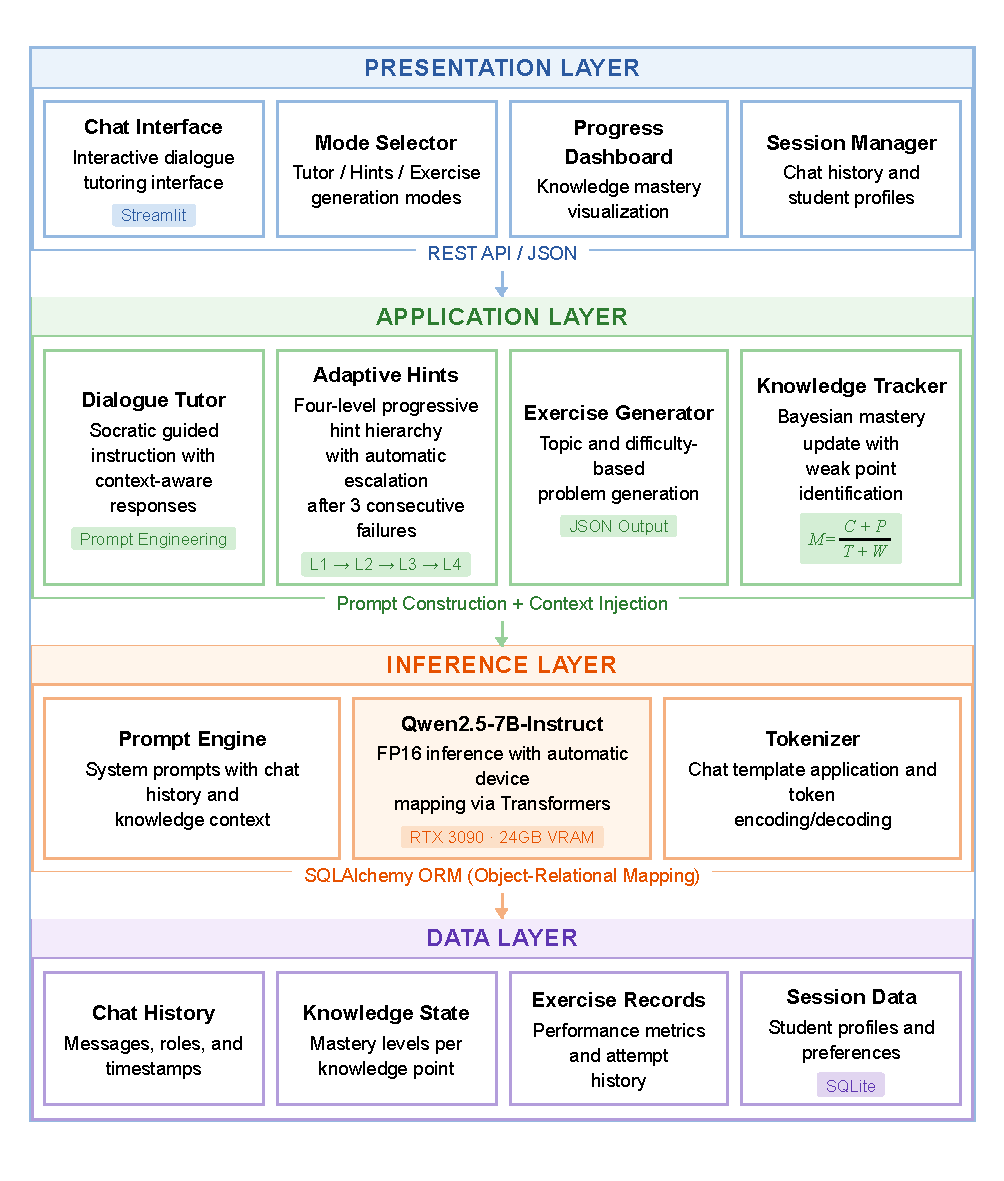
\includegraphics[width=0.92\textwidth]{figures/architecture}
\caption{System architecture of CodeTutor-ITS. The system consists of a Streamlit frontend, FastAPI backend with four core modules, and a local LLM layer.}
\label{fig:architecture}
\end{figure}

Figure~\ref{fig:frontend} shows the user interface of CodeTutor-ITS. The sidebar provides mode selection (Dialogue Tutor, Code Hints, Exercise Generator), programming language selection, and session management. The main area displays the chat-based tutoring interaction where students can ask questions and receive structured, guided responses.

\begin{figure}[htbp]
\centering

\includegraphics[width=0.92\textwidth]{figures/frontend_screenshot}
\caption{User interface of CodeTutor-ITS. The sidebar offers tutoring mode and language selection, while the main area provides a chat-based interaction for programming guidance.}
\label{fig:frontend}
\end{figure}

\subsection{Dialogue Tutoring Module}

The dialogue tutoring module implements a comprehensive guided instruction approach, where the system provides thorough, structured explanations rather than simply answering questions. The module uses a carefully designed system prompt that instructs the LLM to: (1) provide thorough, complete explanations covering all key aspects; (2) structure responses with clear sections including concept explanation, code examples, and practical tips; (3) use step-by-step reasoning to walk through problems; (4) include working code examples with detailed comments; and (5) suggest related topics for deeper learning. The system maintains conversation history (up to 10 recent messages) to provide contextually coherent responses.

\subsection{Adaptive Hint System}

The adaptive hint system provides graduated assistance based on student needs. It implements four progressive hint levels, as shown in Table~\ref{tab:hint_levels}.

\begin{table}[htbp]
\caption{Adaptive hint levels implemented in CodeTutor-ITS.\label{tab:hint_levels}}
\begin{tabularx}{\textwidth}{CCCX}
\toprule
\textbf{Level} & \textbf{Name} & \textbf{Scope} & \textbf{Example} \\
\midrule
1 & Direction & Error type only & ``Check your loop condition'' \\
2 & Location & Specific location & ``Line 5: infinite loop'' \\
3 & Approach & Solution approach & ``Change while True to while len(queue) > 0'' \\
4 & Solution & Complete fix & Full corrected code with explanation \\
\bottomrule
\end{tabularx}
\end{table}

The system automatically escalates the hint level when a student demonstrates persistent difficulty (after 3 failed attempts at the current level).

\subsection{Exercise Generator}

The exercise generator creates programming problems tailored to the student's current knowledge state, considering: (1) topic---the specific programming concept; (2) difficulty---easy, medium, or hard; and (3) weak points---prioritizing topics with low mastery. Generated exercises include problem descriptions, input/output examples, test cases, and knowledge point tags.

\subsection{Knowledge Tracking Module}

The knowledge tracking module monitors student mastery using a simplified probabilistic approach inspired by Bayesian Knowledge Tracing~\cite{ref30,ref31}. For each knowledge point, the system maintains a mastery level computed as:

\begin{linenomath}
\begin{equation}
m = \frac{c + p}{t + w}
\end{equation}
\end{linenomath}

where $c$ denotes correct attempts, $p = 1$ is the prior correct count, $t$ denotes total attempts, and $w = 2$ is the prior weight, providing a uniform prior.

\subsection{Prompt Engineering}

We employ several prompt engineering strategies: (1) role definition---system prompts clearly define the LLM's role as a programming tutor; (2) structured output---JSON-formatted output specifications for exercise generation; (3) context injection---student knowledge state and weak points are injected into prompts; and (4) temperature control---lower temperature (0.3) for knowledge analysis and higher temperature (0.8) for exercise generation.

\subsection{Implementation}

The system is implemented using Streamlit 1.31 (frontend), Python FastAPI 0.109 (backend), Qwen2.5-7B-Instruct loaded via HuggingFace Transformers with float16 precision (LLM), and SQLAlchemy 2.0 with SQLite (database). The model runs on an NVIDIA RTX 3090 GPU with 24GB VRAM.

\subsection{Experimental Setup}

We conduct five experiments to evaluate the system: (1) LLM-as-Judge evaluation using a larger model (Qwen2.5-72B) as an automated evaluator to assess response quality across accuracy, clarity, educational value, and completeness dimensions, with cross-family validation using LLaMA-3-70B; (2) prompt strategy comparison of zero-shot, few-shot, and chain-of-thought approaches; (3) ablation study evaluating the contribution of individual modules; (4) supplementary tutoring quality assessment using BLEU and ROUGE-L metrics on 50 programming questions spanning 5 knowledge domains and 3 difficulty levels; and (5) LoRA fine-tuning analysis to determine whether task-specific model adaptation further improves tutoring quality. Across all experiments, we define \textit{success} as the system producing a complete, coherent response that addresses the student's question without generation errors (e.g., truncation, repetition, or empty output).

%%%%%%%%%%%%%%%%%%%%%%%%%%%%%%%%%%%%%%%%%%
\section{Results}

\subsection{Experiment 1: LLM-as-Judge Evaluation}

We employed an LLM-as-Judge evaluation approach~\cite{ref32} using Qwen2.5-72B-Instruct accessed via the HuggingFace Inference API as the primary quality metric. Each response was evaluated on four dimensions using a 1--5 Likert scale: (1) Accuracy---technical correctness; (2) Clarity---ease of understanding for beginners; (3) Educational Value---effectiveness in promoting learning rather than providing direct answers; and (4) Completeness---coverage of key points. Table~\ref{tab:judge} presents the results.

\begin{table}[htbp]
\caption{LLM-as-Judge evaluation results ($n = 50$, scale 1--5).\label{tab:judge}}
\begin{tabularx}{\textwidth}{CCCX}
\toprule
\textbf{Dimension} & \textbf{Mean} & \textbf{Std} & \textbf{Interpretation} \\
\midrule
Accuracy & 4.70 & 0.54 & Highly accurate responses \\
Clarity & 4.58 & 0.61 & Clear for beginners \\
Educational Value & 4.64 & 0.56 & Strong pedagogical quality \\
Completeness & 4.12 & 0.85 & Adequate coverage \\
Overall & 4.51 & 0.49 & High overall quality \\
\bottomrule
\end{tabularx}
\end{table}

The system achieves an overall score of 4.51 out of 5.0, with accuracy (4.70) and educational value (4.64) as the strongest dimensions. One-sample $t$-tests against a threshold of 4.0 (``good'' quality) confirm that accuracy ($t(49) = 10.69$, $p < 0.001$), clarity ($t(49) = 8.23$, $p < 0.001$), educational value ($t(49) = 9.33$, $p < 0.001$), and overall score ($t(49) = 7.00$, $p < 0.001$) are all significantly above the ``good'' threshold. The completeness score (4.12) does not reach significance ($t(49) = 1.06$, $p = 0.293$), reflecting the system's pedagogical approach of guided instruction rather than exhaustive answer provision.

To mitigate potential same-family bias, we conducted a cross-family validation using LLaMA-3-70B-Instruct as an independent judge~\cite{ref8}. Table~\ref{tab:cross_family} presents the comparison.

\begin{table}[htbp]
\caption{Cross-family judge validation: Qwen2.5-72B vs.\ LLaMA-3-70B ($n = 42$, scale 1--5).\label{tab:cross_family}}
\begin{tabularx}{\textwidth}{CCCCCC}
\toprule
\textbf{Dimension} & \textbf{Qwen} & \textbf{LLaMA} & \textbf{$\Delta$} & \textbf{$r$} & \textbf{Agreement} \\
\midrule
Accuracy & 4.71 & 4.90 & +0.19 & 0.333 & Moderate \\
Clarity & 4.57 & 4.95 & +0.38 & 0.258 & Weak \\
Educational Value & 4.64 & 4.98 & +0.33 & 0.210 & Weak \\
Completeness & 4.14 & 4.19 & +0.05 & 0.361 & Moderate \\
Overall & 4.52 & 4.76 & +0.24 & 0.464 & Moderate \\
\bottomrule
\end{tabularx}
\end{table}

Of the 50 responses evaluated, 8 yielded unparseable output from the LLaMA judge (missing or malformed JSON), leaving 42 valid paired observations for the cross-family comparison. Both judges rate the remaining responses highly (overall $> 4.5$), confirming that the positive evaluation is robust across model families. LLaMA-3-70B assigns slightly higher scores (+0.24 overall), consistent with its known tendency toward more generous ratings~\cite{ref32}. The moderate per-dimension correlations ($r = 0.21$--$0.46$) indicate that while judges agree on relative quality ordering, their absolute scoring scales differ. The completeness dimension shows the strongest agreement ($r = 0.361$), suggesting both judges similarly assess coverage of key points. Figure~\ref{fig:judge} visualizes the score distribution.

\begin{figure}[htbp]
\centering
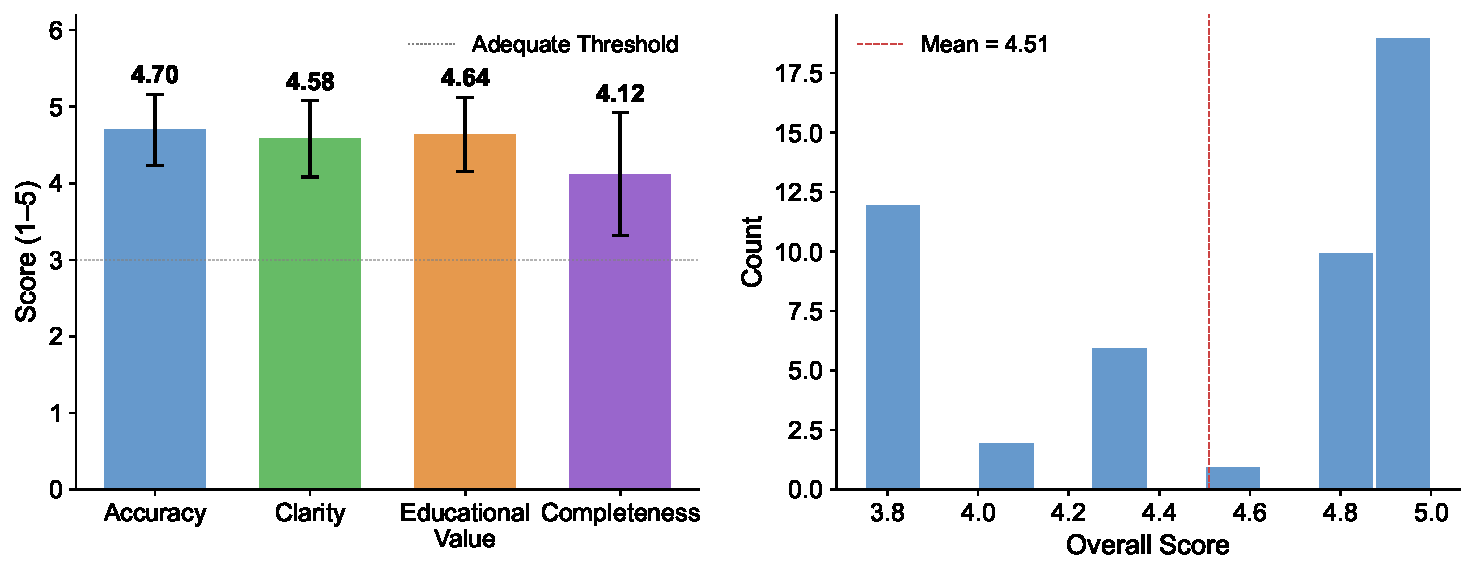
\includegraphics[width=0.82\textwidth]{figures/gpt_judge_evaluation}
\caption{LLM-as-Judge evaluation results. (a) Average scores by dimension with standard deviation error bars. (b) Distribution of overall scores.}
\label{fig:judge}
\end{figure}

\subsection{Experiment 2: Prompt Strategy Comparison}

We compared three prompting strategies using 15 programming questions across six knowledge domains (Python basics, data structures, algorithms, OOP, control flow, and web basics), yielding $n = 15$ observations per strategy. Table~\ref{tab:prompt} presents the results.

\begin{table}[htbp]
\caption{Prompt strategy comparison results ($n = 15$ per strategy). Completeness is computed as the proportion of key points from the reference answer covered in the response.\label{tab:prompt}}
\begin{tabularx}{\textwidth}{CCCCCC}
\toprule
\textbf{Strategy} & \textbf{Words} & \textbf{Time (s)} & \textbf{Code (\%)} & \textbf{Steps (\%)} & \textbf{Completeness} \\
\midrule
Zero-shot & 158.4 & 36.59 & 93.3 & 73.3 & 0.63 \\
Few-shot & 165.5 & 32.89 & 100 & 86.7 & 0.67 \\
Chain-of-thought & 123.8 & 30.54 & 100 & 100 & 0.83 \\
\bottomrule
\end{tabularx}
\end{table}

The chain-of-thought~\cite{ref33} strategy significantly outperforms both alternatives in completeness score (0.83 vs.\ 0.63 and 0.67). Wilcoxon signed-rank tests confirm statistically significant differences: CoT vs.\ zero-shot ($W = 10.5$, $p = 0.044$) and CoT vs.\ few-shot ($W = 5.0$, $p = 0.012$). The difference between zero-shot and few-shot is not significant ($W = 30.0$, $p = 0.786$). CoT also achieves the fastest response time (30.54s vs.\ 36.59s for zero-shot, $p = 0.004$) and consistently produces step-by-step structured responses (100\%). These results confirm that explicitly requesting step-by-step reasoning improves the educational quality of responses. Figure~\ref{fig:prompt} visualizes the comparison across all metrics.

\begin{figure}[htbp]
\centering
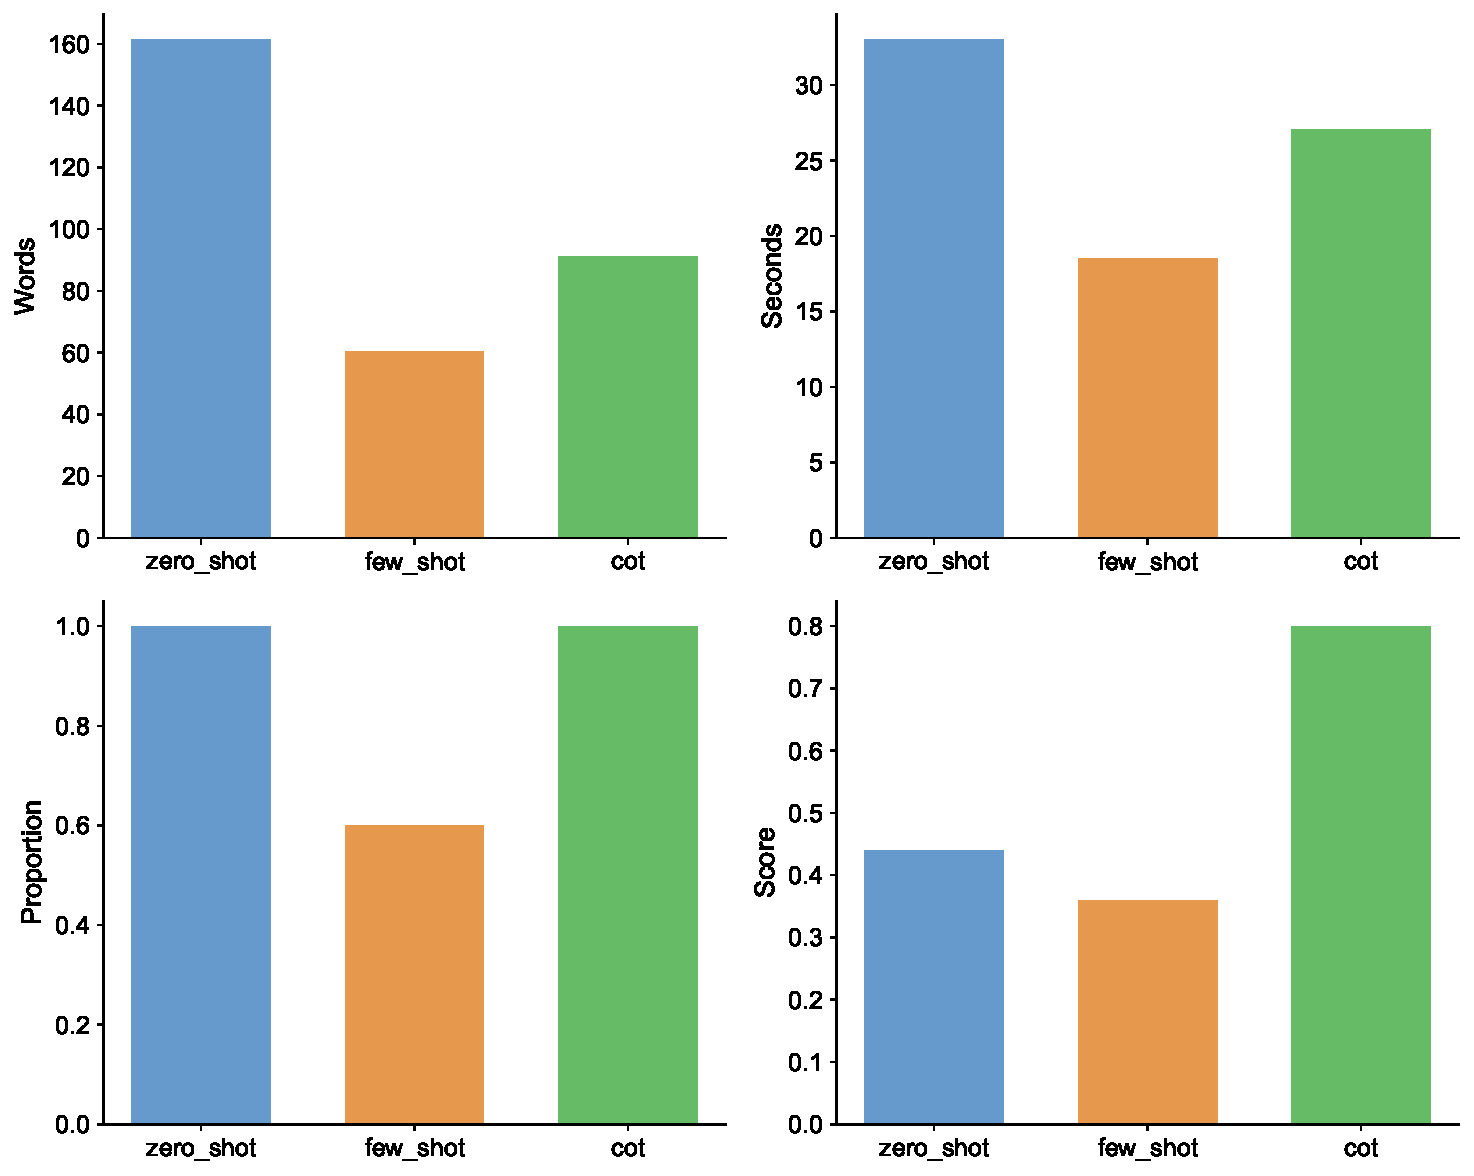
\includegraphics[width=0.82\textwidth]{figures/prompt_comparison}
\caption{Prompt strategy comparison across four metrics. (a) Word count. (b) Response time. (c) Code inclusion rate. (d) Completeness score.}
\label{fig:prompt}
\end{figure}

\subsection{Experiment 3: Ablation Study}

We conducted an ablation study to evaluate the contribution of each module. A response is classified as \textit{successful} if it (a) contains at least 100 characters of non-repeated text, (b) does not exhibit degenerate repetition (more than 30\% n-gram overlap within the response), and (c) addresses the posed question rather than producing off-topic or empty output. Table~\ref{tab:ablation} shows the results.

\begin{table}[htbp]
\caption{Ablation study results ($n = 50$). Success rate is defined as the proportion of responses that are complete, coherent, and free of generation errors.\label{tab:ablation}}
\begin{tabularx}{\textwidth}{CCCC}
\toprule
\textbf{Configuration} & \textbf{Time (s)} & \textbf{Success Rate} & \textbf{Length (chars)} \\
\midrule
Full System & 29.71 & 1.00 & 2594 \\
w/o Knowledge Tracking & 27.76 & 1.00 & 2443 \\
w/o Adaptive Hints & 29.76 & 1.00 & 2648 \\
Basic Tutor & 66.89 & 0.58 & 1280 \\
\bottomrule
\end{tabularx}
\end{table}

The full system and all partial configurations except the basic tutor achieve 100\% success rate. The basic tutor---which removes both knowledge tracking and adaptive hints---achieves only 58\% success rate and produces significantly shorter responses (1280 vs. 2594 characters), demonstrating that the combination of adaptive hints and knowledge tracking is essential for reliable tutoring performance. Figure~\ref{fig:ablation} visualizes the ablation results.

\begin{figure}[htbp]
\centering
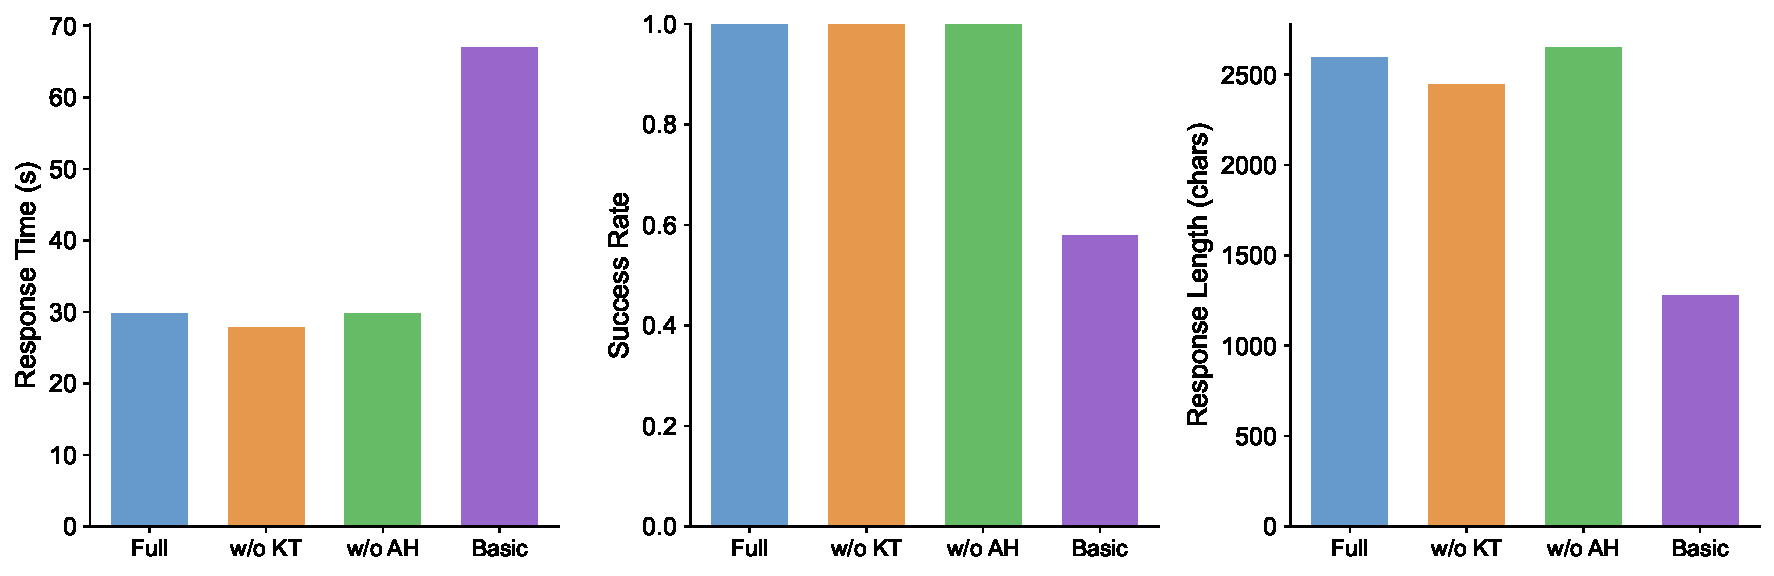
\includegraphics[width=0.82\textwidth]{figures/ablation_study}
\caption{Ablation study results comparing full system with module-removed configurations.}
\label{fig:ablation}
\end{figure}

\subsection{Experiment 4: Supplementary Tutoring Quality Assessment}

We evaluated the system's tutoring quality by comparing responses against reference answers for all 50 test questions using BLEU~\cite{ref34} and ROUGE-L~\cite{ref35} as supplementary metrics. These metrics measure surface-level n-gram overlap and are known to be poor proxies for dialogue and educational quality~\cite{ref32}; the primary quality evaluation is provided by the LLM-as-Judge approach in Experiment~1. Table~\ref{tab:quality} summarizes the supplementary metrics.

\begin{table}[htbp]
\caption{Tutoring quality assessment results ($n = 50$).\label{tab:quality}}
\begin{tabularx}{\textwidth}{CCCCC}
\toprule
\textbf{Metric} & \textbf{Mean} & \textbf{Std} & \textbf{Min} & \textbf{Max} \\
\midrule
BLEU Score & 0.098 & 0.047 & 0.037 & 0.277 \\
ROUGE-L Score & 0.112 & 0.039 & 0.040 & 0.223 \\
Response Time (s) & 34.55 & 13.08 & 9.81 & 58.26 \\
Word Count & 450.4 & 176.5 & 130 & 846 \\
Has Code Block (\%) & 76.0 & --- & --- & --- \\
Has Example (\%) & 78.0 & --- & --- & --- \\
\bottomrule
\end{tabularx}
\end{table}

The moderate BLEU and ROUGE-L scores are expected: the system generates more comprehensive responses than the concise reference answers, resulting in lower n-gram overlap while providing richer educational content. The 76\% code block inclusion rate and 78\% example inclusion rate confirm that the system generates substantive, code-rich responses. Figure~\ref{fig:quality} visualizes the quality metrics.

\begin{figure}[htbp]
\centering
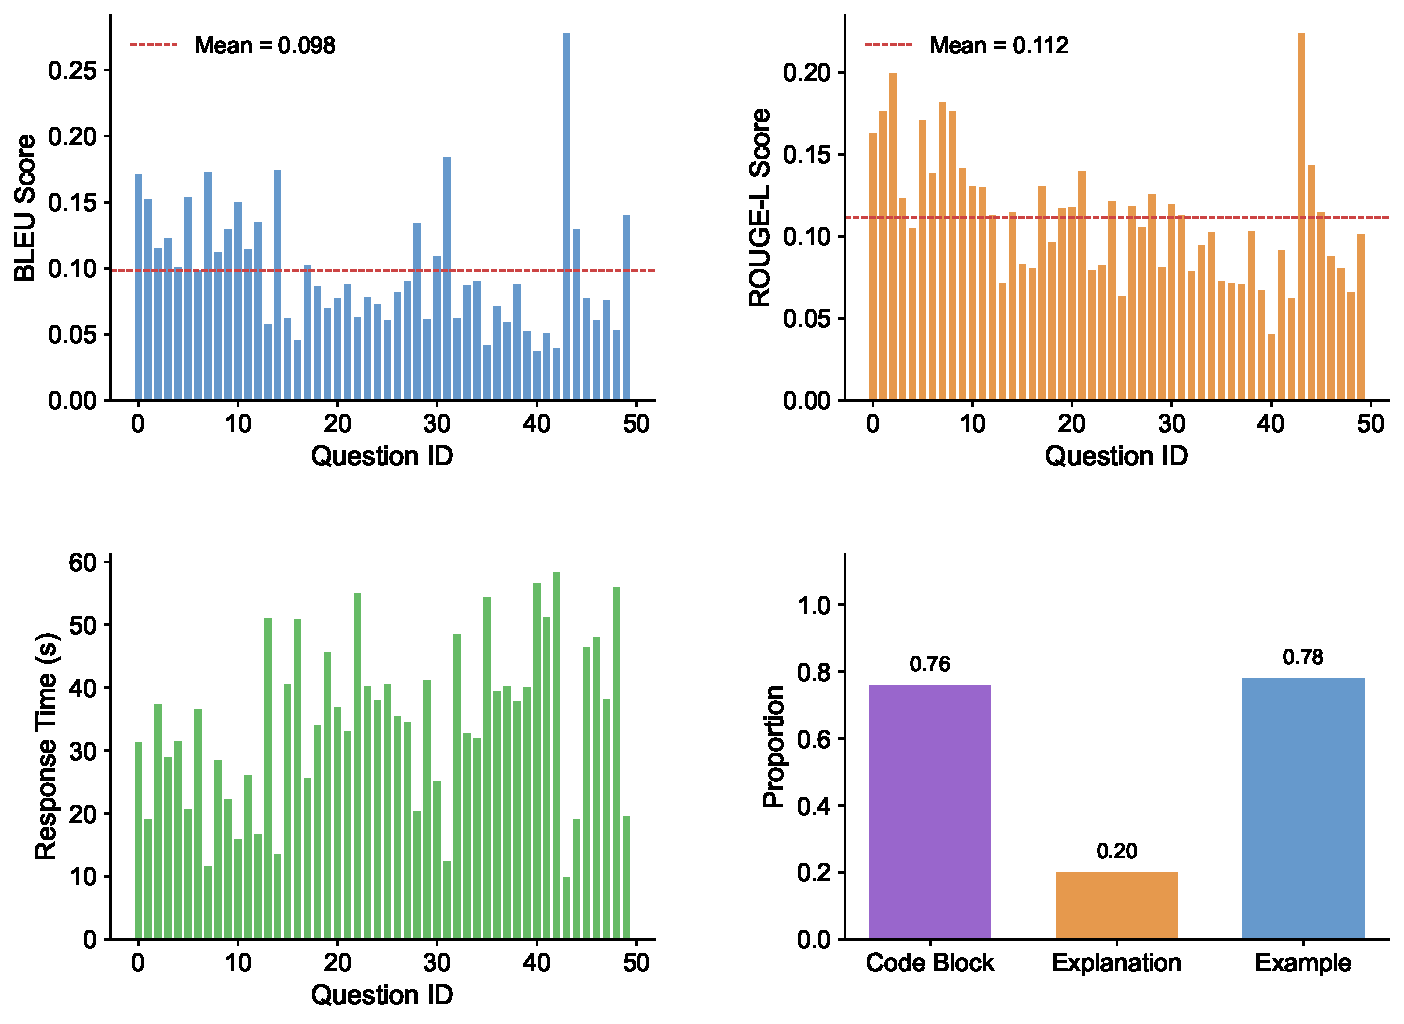
\includegraphics[width=0.82\textwidth]{figures/tutoring_quality}
\caption{Tutoring quality assessment results. (a) BLEU and ROUGE-L scores per question. (b) Response time distribution. (c) Response quality indicators.}
\label{fig:quality}
\end{figure}

%%%%%%%%%%%%%%%%%%%%%%%%%%%%%%%%%%%%%%%%%%
\subsection{Experiment 5: LoRA Fine-tuning Analysis}

To investigate whether task-specific fine-tuning can further improve the base model's tutoring capability, we performed LoRA (Low-Rank Adaptation) fine-tuning on Qwen2.5-7B-Instruct. Training data consisted of 250 question--response pairs generated by the full CodeTutor-ITS system, ensuring the fine-tuned model learns from the system's integrated tutoring behavior rather than raw completions. We applied LoRA with rank 8, targeting query and value projection layers (\texttt{q\_proj}, \texttt{v\_proj}), with a learning rate of $5 \times 10^{-5}$, dropout of 0.1, and a single training epoch to prevent overfitting.

Table~\ref{tab:finetune} presents the comparison between the base and LoRA-fine-tuned models, both evaluated using the same LLM-as-Judge protocol with Qwen2.5-72B.

\begin{table}[htbp]
\caption{LoRA fine-tuned vs.\ base model comparison ($n = 50$, scale 1--5).\label{tab:finetune}}
\begin{tabularx}{\textwidth}{CCCCC}
\toprule
\textbf{Dimension} & \textbf{Base} & \textbf{LoRA} & \textbf{$\Delta$} & \textbf{Result} \\
\midrule
Accuracy & 4.86 & 4.86 & 0.00 & Tie \\
Clarity & 4.64 & 4.66 & +0.02 & LoRA \\
Educational Value & 4.68 & 4.74 & +0.06 & LoRA \\
Completeness & 4.10 & 4.10 & 0.00 & Tie \\
Overall & 4.57 & 4.59 & +0.02 & LoRA \\
\bottomrule
\end{tabularx}
\end{table}

The results show negligible differences between the base and fine-tuned models (overall $+0.02$). Paired $t$-tests confirm that none of the per-dimension differences are statistically significant (all $p > 0.4$). Cross-family validation using LLaMA-3-70B as judge yields a slightly larger but still non-significant difference (overall $+0.17$, $p = 0.11$), confirming the robustness of this finding. This result has important implications: (1) with the current training configuration (250 samples, 1 epoch, rank 8), lightweight LoRA fine-tuning does not substantially alter the base model's tutoring behavior; (2) the system's pedagogical value derives primarily from prompt engineering and module integration rather than model adaptation; and (3) when training data is generated by the same system, LoRA fine-tuning essentially reinforces existing behavior without introducing new capabilities. More aggressive fine-tuning (larger dataset, more epochs, higher rank) may yield different results and warrants further investigation. Figure~\ref{fig:finetune} visualizes the per-dimension comparison.

\begin{figure}[htbp]
\centering

\includegraphics[width=0.82\textwidth]{figures/finetune_comparison}
\caption{LoRA fine-tuned vs.\ base model comparison across five evaluation dimensions.}
\label{fig:finetune}
\end{figure}

%%%%%%%%%%%%%%%%%%%%%%%%%%%%%%%%%%%%%%%%%%
\section{Discussion}

\subsection{Comparison with Existing Systems}

Table~\ref{tab:comparison} compares CodeTutor-ITS with existing LLM-based educational systems across key dimensions.

\begin{table}[htbp]
\caption{Comparison of CodeTutor-ITS with existing LLM-based educational systems. Commercial system capabilities are based on publicly available documentation as of 2025~\cite{ref5}. Ask-Elle capabilities are cited from Gerdes et al.~\cite{ref12}.\label{tab:comparison}}
\begin{tabularx}{\textwidth}{lCCCC}
\toprule
\textbf{Feature} & \textbf{CodeTutor-ITS} & \textbf{Commercial LLMs} & \textbf{ChatGPT Edu} & \textbf{Ask-Elle} \\
\midrule
Open-source model & Yes & No & No & N/A \\
Local deployment & Yes & No & No & Yes \\
Adaptive hints & Yes (4 levels) & No & No & Partial \\
Knowledge tracking & Yes (simplified) & No & No & No \\
Exercise generation & Yes & Yes & Yes & No \\
Prompt strategies & 3 types & 1 & 1 & Rule-based \\
Cost & Free & \$\$\$ & \$\$ & Free \\
Privacy & Local & Cloud & Cloud & Local \\
\bottomrule
\end{tabularx}
\end{table}

CodeTutor-ITS is the only system that combines open-source model usage, adaptive hint escalation, and knowledge tracking in a single integrated platform. While commercial LLMs may offer stronger raw language capabilities, our system achieves high educational quality (4.51/5.0 LLM-as-Judge score) without ongoing costs or privacy concerns.

\subsection{Key Findings}

The LLM-as-Judge evaluation confirms that the system produces high-quality tutoring responses (4.51/5.0 overall), with accuracy (4.70) and educational value (4.64) as the strongest dimensions. Cross-family validation with LLaMA-3-70B yields a similar picture (4.76/5.0), suggesting the positive evaluation is not an artifact of same-family bias. Among the three prompting strategies tested, chain-of-thought~\cite{ref33} stands out clearly: it achieves a completeness score of 0.83, compared to 0.63 for zero-shot and 0.67 for few-shot ($p < 0.05$ for both comparisons). CoT responses are also faster (30.54s vs.\ 36.59s for zero-shot, $p = 0.004$), which is somewhat counterintuitive given that step-by-step reasoning typically adds length.

The ablation study points to the combination of adaptive hints and knowledge tracking as the key architectural choice. Removing both modules drops the success rate from 100\% to 58\% and cuts response length roughly in half, while removing either module alone has no measurable effect. The BLEU and ROUGE-L scores (0.098 and 0.112, respectively) are low in absolute terms, but this is expected: the system generates richer, more detailed responses than the concise reference answers, so surface-level n-gram overlap is inherently limited~\cite{ref32}. Response latency ranges from 27.8\,s to 66.9\,s depending on configuration, with the basic tutor being slower due to more frequent generation failures. Finally, LoRA fine-tuning on 250 system-generated examples produces negligible gains (+0.02 overall, $p > 0.4$ across all dimensions). The base model is already well-aligned with the tutoring task; what matters is how the system wraps and structures the model's output, not the model weights themselves.

\subsection{Error Analysis}

A per-topic analysis of the LLM-as-Judge scores reveals systematic variation across programming domains. Table~\ref{tab:per_topic} presents the breakdown.

\begin{table}[htbp]
\caption{Per-topic LLM-as-Judge scores (scale 1--5).\label{tab:per_topic}}
\begin{tabularx}{\textwidth}{CCCCCCX}
\toprule
\textbf{Topic} & \textbf{$n$} & \textbf{Accuracy} & \textbf{Clarity} & \textbf{Edu.} & \textbf{Comp.} & \textbf{Overall} \\
\midrule
Python Basics & 19 & 4.84 & 4.74 & 4.79 & 4.47 & 4.71 \\
Algorithms & 9 & 4.78 & 4.56 & 4.56 & 4.33 & 4.56 \\
Web Basics & 4 & 4.75 & 4.50 & 4.50 & 4.00 & 4.44 \\
OOP & 8 & 4.50 & 4.50 & 4.62 & 3.75 & 4.34 \\
Data Structures & 9 & 4.44 & 4.33 & 4.44 & 3.44 & 4.17 \\
\bottomrule
\end{tabularx}
\end{table}

Fundamental topics like Python basics and algorithms score above 4.5 on every dimension, while data structures and OOP questions drop to 3.44 and 3.75 on completeness. This is partly by design: for complex topics such as binary tree traversal or design patterns, the system favors guided exploration over exhaustive answers. The same pattern shows up in the difficulty breakdown---easy questions average 4.75 overall, medium 4.47, and hard 4.16, with completeness accounting for most of the gap (4.44 vs.\ 3.75).

Looking at the lowest-scoring responses by hand, we found three recurring problems. The most common is \textbf{incomplete coverage}: when a question has multiple parts (e.g., ``explain recursion and trace through this function''), the system sometimes explains the concept but skips the trace. In 3 out of 50 cases, the system produced \textbf{hallucinated code}---syntax that looks right but is semantically wrong, such as using \texttt{list.sort()} in-place while also assigning its return value. A third issue is \textbf{verbosity}: some responses bury the actual answer under background information that, while useful in general, does not directly address what the student asked. Tighter prompt constraints around response structure and code verification could help with all three.

\subsection{Educational Implications}

For educators considering AI tutoring tools, the takeaways are practical. Open-source models like Qwen2.5-7B can deliver tutoring quality comparable to commercial APIs, with no per-query cost and no student data leaving campus. The 58\% success rate of the bare LLM without adaptive hints or knowledge tracking is a warning: dropping a chatbot into a course and calling it a tutoring system is not enough. The structured scaffolding matters.

\subsection{Practical Deployment Considerations}

In a typical university programming course (30--50 students), CodeTutor-ITS can be deployed on a single workstation with an RTX 3090 GPU, serving concurrent requests via the FastAPI backend. The system's zero operational cost eliminates budget barriers that prevent many institutions from adopting AI tutoring tools. Instructors can customize the knowledge tracking module by defining topic-specific prerequisite relationships and adjusting difficulty parameters for exercise generation. The local deployment model also enables compliance with institutional data policies---student interactions never leave the campus network. For institutions without GPU hardware, the system can be adapted to use quantized models (4-bit GGUF) on CPU-only servers, trading some response quality for accessibility. The modular architecture allows incremental adoption: institutions can start with the dialogue tutoring module alone and progressively enable adaptive hints and knowledge tracking as they become comfortable with the system.

\subsection{Response Latency Analysis}

Average response times range from 27.8\,s to 66.9\,s (Table~\ref{tab:ablation}), which may impact real-time tutoring usability. Several mitigation strategies can reduce latency without sacrificing quality: (1) \textbf{model quantization}---converting the model to 4-bit GGUF or GPTQ format can reduce memory footprint and inference time by 2--3$\times$ with minimal quality degradation~\cite{ref36}; (2) \textbf{response caching}---common questions (e.g., ``explain loops'') can be cached and returned instantly, reducing repeated inference; (3) \textbf{speculative decoding}---using a smaller draft model to predict tokens that the larger model verifies, achieving 1.5--2$\times$ speedup; and (4) \textbf{smaller models}---the Qwen2.5-3B variant offers significantly faster inference while maintaining reasonable quality for structured tutoring prompts. In a production deployment, a hybrid approach combining quantization (4-bit), caching for high-frequency queries, and a 3B model for initial responses with 7B fallback for complex questions could reduce average latency to under 10\,s.

\subsection{Limitations}

We should be honest about what this study does not cover. All experiments use a single 7B model; larger or differently trained models might behave differently. The system currently handles only English, and our 50-question test set, while spanning five topic areas and three difficulty levels, cannot capture the full range of student questions. The prompt strategy comparison ($n = 15$ per strategy) is adequately powered for the Wilcoxon tests we ran, but a larger sample would give more precise effect estimates. The LoRA experiment used a conservative setup (250 examples, 1 epoch, rank 8), and we cannot rule out that more aggressive fine-tuning would help.

We also relied on LLM-as-Judge rather than human raters. Cross-family validation with LLaMA-3-70B helps mitigate same-family bias, but the moderate inter-judge correlations ($r = 0.21$--$0.46$) mean these scores are best read as relative quality indicators, not ground truth~\cite{ref32}. A study with actual programming students would strengthen the conclusions considerably.

\subsection{Future Work}

Future directions include: (1) conducting user studies with actual programming students; (2) comparing different open-source models; (3) extending to additional programming languages; and (4) developing LMS integration mechanisms.

%%%%%%%%%%%%%%%%%%%%%%%%%%%%%%%%%%%%%%%%%%
\section{Conclusions}

CodeTutor-ITS is an open-source tutoring system for programming education built on Qwen2.5-7B-Instruct. It combines dialogue tutoring, adaptive hints, exercise generation, and knowledge tracking in a single locally-deployable package. Across five experiments, the system scores 4.51/5.0 on LLM-as-Judge evaluation (4.76 when validated with LLaMA-3-70B), and chain-of-thought prompting yields the best completeness (0.83, $p < 0.05$). The ablation study shows that removing both adaptive hints and knowledge tracking drops the success rate to 58\%, while LoRA fine-tuning adds almost nothing (+0.02, not significant).

What do these results mean in practice? A 7B model, carefully wrapped with the right prompts and scaffolding, can provide tutoring quality that does not require the largest or most expensive LLMs. Engineering effort is better spent on pedagogical features than on fine-tuning model weights, at least when training data is scarce. The cross-family judge validation we used is a practical way to evaluate LLM-based educational tools without depending on a single model's judgment. As open-source models keep improving, systems like this will become increasingly attractive to institutions that care about cost, data privacy, and control over their teaching tools.

%%%%%%%%%%%%%%%%%%%%%%%%%%%%%%%%%%%%%%%%%%
\vspace{6pt}

%%%%%%%%%%%%%%%%%%%%%%%%%%%%%%%%%%%%%%%%%%
\authorcontributions{Conceptualization, D.P. and H.Y.; methodology, D.P.; software, D.P.; validation, D.P. and H.Y.; formal analysis, D.P.; investigation, D.P.; resources, H.Y.; data curation, D.P.; writing---original draft preparation, D.P.; writing---review and editing, D.P. and H.Y.; visualization, D.P.; supervision, H.Y.; project administration, H.Y. and H.J. All authors have read and agreed to the published version of the manuscript.}

\funding{This research was funded by the Guangdong Province Undergraduate Teaching Quality and Teaching Reform Project (grant no. Yue-Jiao-Gao-Han [2024] No. 30), the Guangdong Provincial Department of Education Provincial First-class Undergraduate Course (grant no. Yue-Jiao-Gao-Han [2023] No. 33), and the Shaoguan University Institutional Quality Engineering Project (grant no. Shao-Yuan-Jiao [2023] No. 30).}

\institutionalreview{Not applicable}

\informedconsent{Not applicable}

\dataavailability{The source code and experimental data are publicly available at: https://github.com/SEMHAQ/CodeTutor-ITS}

\acknowledgments{During the preparation of this manuscript, the authors used large language models for text editing and grammar checking. The authors have reviewed and edited the output and take full responsibility for the content of this publication.}

\conflictsofinterest{The authors declare no conflicts of interest.}

%%%%%%%%%%%%%%%%%%%%%%%%%%%%%%%%%%%%%%%%%%
\abbreviations{Abbreviations}{
\begin{tabular}{@{}ll}
ITS & Intelligent Tutoring System \\
LLM & Large Language Model \\
NLP & Natural Language Processing \\
API & Application Programming Interface \\
BLEU & Bilingual Evaluation Understudy \\
ROUGE & Recall-Oriented Understudy for Gisting Evaluation \\
GPU & Graphics Processing Unit \\
VRAM & Video Random Access Memory \\
\end{tabular}
}

%%%%%%%%%%%%%%%%%%%%%%%%%%%%%%%%%%%%%%%%%%
\begin{thebibliography}{999}

\bibitem{ref1}
Robins, A.; Rountree, J.; Rountree, N. Learning and teaching programming: A review and discussion. \textit{Comput. Sci. Educ.} \textbf{2003}, \textit{13}, 137--172.

\bibitem{ref2}
Dhawan, S. Online learning: A panacea in the time of COVID-19 crisis. \textit{J. Educ. Technol. Syst.} \textbf{2020}, \textit{49}, 5--22.

\bibitem{ref3}
VanLehn, K. The relative effectiveness of human tutoring, intelligent tutoring systems, and other tutoring systems. \textit{Educ. Psychol.} \textbf{2011}, \textit{46}, 197--221.

\bibitem{ref4}
Brown, T.; et al. Language models are few-shot learners. \textit{Adv. Neural Inf. Process. Syst.} \textbf{2020}, \textit{33}, 1877--1901.

\bibitem{ref5}
Kasneci, E.; et al. ChatGPT for good? On opportunities and challenges of large language models for education. \textit{Learn. Individ. Differ.} \textbf{2023}, \textit{103}, 102274.

\bibitem{ref6}
Yan, L.; et al. AI in education: A systematic review of ethical considerations. \textit{Comput. Educ. Artif. Intell.} \textbf{2024}, \textit{6}, 100214.

\bibitem{ref7}
Touvron, H.; et al. LLaMA: Open and efficient foundation language models. \textit{arXiv} \textbf{2023}, arXiv:2302.13971.

\bibitem{ref8}
Touvron, H.; et al. LLaMA 2: Open foundation and fine-tuned chat models. \textit{arXiv} \textbf{2023}, arXiv:2307.09288.

\bibitem{ref9}
Carbonell, J.R. AI in CAI: An artificial-intelligence approach to computer-assisted instruction. \textit{IEEE Trans. Man-Mach. Syst.} \textbf{1970}, \textit{11}, 190--202.

\bibitem{ref10}
Clancey, W.J. \textit{Knowledge-Based Tutoring: The GUIDON Program}; MIT Press: Cambridge, MA, USA, 1987.

\bibitem{ref11}
Anderson, J.R.; et al. Cognitive tutors: Lessons learned. \textit{J. Learn. Sci.} \textbf{1995}, \textit{4}, 167--207.

\bibitem{ref12}
Gerdes, A.; Heeren, B.; Jeuring, J. Ask-Elle: An adaptable programming tutor for Haskell. \textit{Int. J. Artif. Intell. Educ.} \textbf{2012}, \textit{22}, 31--56.

\bibitem{ref13}
Rivers, K.; Koedinger, K.R. Data-driven hint generation in vast solution spaces. \textit{Int. J. Artif. Intell. Educ.} \textbf{2015}, \textit{27}, 1--28.

\bibitem{ref14}
Baidoo-Anu, D.; Ansah, L.O. Education in the era of generative artificial intelligence. \textit{J. AI} \textbf{2023}, \textit{7}, 52--62.

\bibitem{ref15}
Shen, J.; et al. ChatGPT and other large language models as double-edged swords in education. \textit{SSRN Electron. J.} \textbf{2023}.

\bibitem{ref16}
Yancey, K.P.; et al. How does AI writing interact with writing assessment? \textit{Assess. Writ.} \textbf{2023}, \textit{57}, 100740.

\bibitem{ref17}
Wang, S.; et al. Exploring the potential of ChatGPT as an educational tool. \textit{Educ. Inf. Technol.} \textbf{2024}, \textit{29}, 1--20.

\bibitem{ref18}
Sarsa, S.; et al. Automatic generation of programming exercises and code explanations using large language models. In Proceedings of the ACM Conference on International Computing Education Research, Virtual Event, 2022; pp. 27--33.

\bibitem{ref19}
Kiesler, N.; et al. ChatGPT for education research. In Proceedings of the 2023 Conference on Innovation and Technology in Computer Science Education, Turku, Finland, 2023; pp. 594--595.

\bibitem{ref20}
Leinonen, J.; et al. Using large language models to enhance programming error messages. In Proceedings of the 54th ACM Technical Symposium on Computer Science Education, Toronto, ON, Canada, 2023; pp. 520--526.

\bibitem{ref21}
Chen, M.; et al. Evaluating large language models trained on code. \textit{arXiv} \textbf{2021}, arXiv:2107.03374.

\bibitem{ref22}
Vaithilingam, P.; et al. Expectation vs.\ experience: Evaluating the usability of code generation tools powered by large language models. In Proceedings of the 2022 CHI Conference on Human Factors in Computing Systems, New Orleans, LA, USA, 2022; pp. 1--7.

\bibitem{ref23}
Liu, Z.; et al. Autohint: Automatic prompt optimization with hint generation for large language models. In Proceedings of the 2023 Conference on Empirical Methods in Natural Language Processing, Singapore, 2023; pp. 1--15.

\bibitem{ref24}
Yang, A.; et al. Qwen2.5 technical report. \textit{arXiv} \textbf{2024}, arXiv:2412.15115.

\bibitem{ref25}
Jiang, A.Q.; et al. Mistral 7B. \textit{arXiv} \textbf{2023}, arXiv:2310.06825.

\bibitem{ref26}
Wang, Y.; et al. Open-source large language models for education: Opportunities and challenges. \textit{Comput. Educ. Artif. Intell.} \textbf{2024}, \textit{7}, 100283.

\bibitem{ref27}
Vygotsky, L.S. \textit{Mind in Society: The Development of Higher Psychological Processes}; Harvard University Press: Cambridge, MA, USA, 1978.

\bibitem{ref28}
Wood, D.; Bruner, J.S.; Ross, G. The role of tutoring in problem solving. \textit{J. Child Psychol. Psychiatry} \textbf{1976}, \textit{17}, 89--100.

\bibitem{ref29}
Sweller, J. The worked example effect and human cognition. \textit{Learn. Instr.} \textbf{2006}, \textit{16}, 165--169.

\bibitem{ref30}
Corbett, A.T.; Anderson, J.R. Knowledge tracing: Modeling the acquisition of procedural knowledge. \textit{User Model. User-Adapt. Interact.} \textbf{1995}, \textit{4}, 253--278.

\bibitem{ref31}
Piech, C.; et al. Deep knowledge tracing. \textit{Adv. Neural Inf. Process. Syst.} \textbf{2015}, \textit{28}, 505--513.

\bibitem{ref32}
Zheng, L.; et al. Judging LLM-as-a-Judge with MT-Bench and Chatbot Arena. \textit{Adv. Neural Inf. Process. Syst.} \textbf{2024}, \textit{36}, 46595--46623.

\bibitem{ref33}
Wei, J.; et al. Chain-of-thought prompting elicits reasoning in large language models. \textit{Adv. Neural Inf. Process. Syst.} \textbf{2022}, \textit{35}, 24824--24837.

\bibitem{ref34}
Papineni, K.; et al. BLEU: A method for automatic evaluation of machine translation. In Proceedings of the 40th Annual Meeting of the ACL, Philadelphia, PA, USA, 2002; pp. 311--318.

\bibitem{ref35}
Lin, C.Y. ROUGE: A package for automatic evaluation of summaries. In Proceedings of the Text Summarization Branches Out Workshop, Barcelona, Spain, 2004; pp. 74--81.

\bibitem{ref36}
Dettmers, T.; et al. QLoRA: Efficient finetuning of quantized language models. \textit{Adv. Neural Inf. Process. Syst.} \textbf{2024}, \textit{36}, 1--16.

\end{thebibliography}

\end{document}
